\documentclass[10pt]{article}
\usepackage[polish]{babel}
\usepackage[utf8]{inputenc}
\usepackage[T1]{fontenc}
\usepackage{amsmath}
\usepackage{amsfonts}
\usepackage{amssymb}
\usepackage[version=4]{mhchem}
\usepackage{stmaryrd}
\usepackage{graphicx}
\usepackage[export]{adjustbox}
\graphicspath{ {./images/} }
\usepackage{hyperref}
\hypersetup{colorlinks=true, linkcolor=blue, filecolor=magenta, urlcolor=cyan,}
\urlstyle{same}

\title{GIMNAZJUM }

\author{}
\date{}


\newcommand\Varangle{\mathop{{<\!\!\!\!\!\text{\small)}}\:}\nolimits}

%New command to display footnote whose markers will always be hidden
\let\svthefootnote\thefootnote
\newcommand\blfootnotetext[1]{%
  \let\thefootnote\relax\footnote{#1}%
  \addtocounter{footnote}{-1}%
  \let\thefootnote\svthefootnote%
}

%Overriding the \footnotetext command to hide the marker if its value is `0`
\let\svfootnotetext\footnotetext
\renewcommand\footnotetext[2][?]{%
  \if\relax#1\relax%
    \ifnum\value{footnote}=0\blfootnotetext{#2}\else\svfootnotetext{#2}\fi%
  \else%
    \if?#1\ifnum\value{footnote}=0\blfootnotetext{#2}\else\svfootnotetext{#2}\fi%
    \else\svfootnotetext[#1]{#2}\fi%
  \fi
}

\begin{document}
\maketitle
\begin{enumerate}
  \item Każdy punkt płaszczyzny pokolorowano na niebiesko lub czerwono. Udowodnij, że istnieje trójkąt prostokątny równoramienny, którego wierzchołki są tego samego koloru.
  \item Znajdź wszystkie liczby całkowite \(n\) takie, że \(\frac{5 n+2}{2 n+3}\) jest liczbą całkowitą.
  \item Dany jest trójkąt \(A B C\), w którym \(\Varangle A=90^{\circ}\) oraz \(A B=A C\). Punkty \(D \mathrm{i} E\) leżą odpowiednio na bokach \(A B\) i \(A C\), przy czym \(A D=C E\). Prosta przechodząca przez punkt \(A\) i prostopadła do prostej \(D E\) przecina bok \(B C\) w punkcie \(P\). Wykaż, że \(A P=D E\).\\
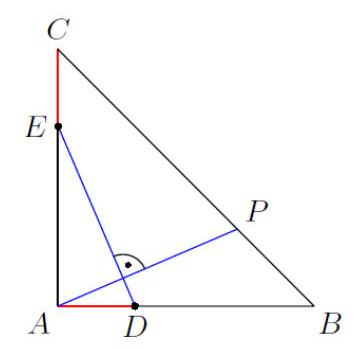
\includegraphics[max width=\textwidth, center]{2024_11_21_3afe6bfe8218957aab49g-1}
\end{enumerate}

\section*{LICEUM}
\begin{enumerate}
  \item Punkty \(E\) i \(F\) leżą odpowiednio na bokach \(A B\) i \(B C\) kwadratu \(A B C D\), przy czym \(B E=B F\). Punkt \(S\) jest rzutem prostokątnym punktu \(B\) na prosta \(C E\). Wykaż, że \(\Varangle D S F=90^{\circ}\).
  \item Dane są różne dodatnie liczby wymierne \(x\) i \(y\), dla których liczba\\
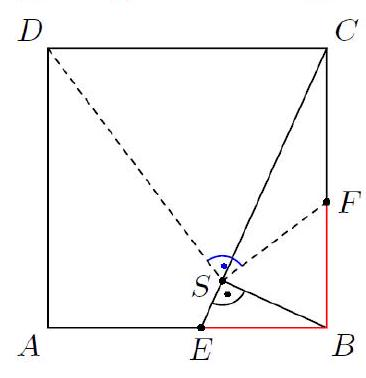
\includegraphics[max width=\textwidth, center]{2024_11_21_3afe6bfe8218957aab49g-1(1)}
\end{enumerate}

\[
w=\frac{x+\sqrt{y}}{y+\sqrt{x}}
\]

jest wymierna. Wykazać, że obie liczby \(x\) i \(y\) są kwadratami liczb wymiernych.\\
3. Wykaż, że jeżeli \(\alpha\) jest kątem ostrym, to

\[
\frac{\frac{1}{(1-\sin \alpha)^{2}}-\frac{1}{(1+\sin \alpha)^{2}}}{\frac{1}{(1-\cos \alpha)^{2}}-\frac{1}{(1+\cos \alpha)^{2}}}=\operatorname{tg}^{5} \alpha
\]

\footnotetext{Rozwiazania należy oddać do piątku 20 maja do godziny 10.35 koordynatorowi konkursu panu Jarosławowi Szczepaniakowi lub swojemu nauczycielowi matematyki lub przestać na adres \href{mailto:jareksz@interia.pl}{jareksz@interia.pl} do piątku 20 maja do pótnocy.
}
\end{document}